\subsection{Ablenkung des Strahls im elektrischen Feld}
\begin{figure}[h]
  \centering
  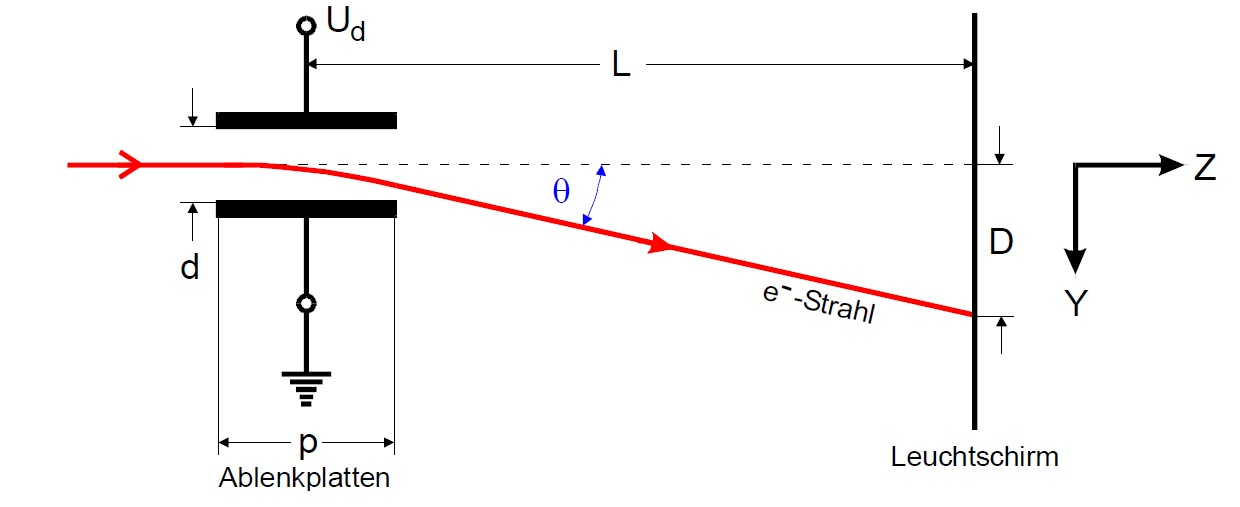
\includegraphics[width=0.7\textwidth]{Grafiken/V501(2)_Abb1.jpg}
  \caption{Strahlablenkung in der Kathodenstrahlröhre \cite{V501}}
\end{figure}
Bewegt sich ein Elektron im homogenen elektrischen Feld wirkt eine Kraft am Elektron. \\
Diese Kraft ist betragsmäßig gleich dem Produkt von Feldstärke und
Ladung:
\begin{equation}
  \label{eq:force}
  |\vec{F}| = |e_0\vec{E}|
\end{equation}

Nach mehreren Umrechnungsschritten ($E = \frac{U_d}{d}$) gilt für die Ablenkgeschwindigkeit $v_{ab}$:
\begin{equation}
  v_{ab} = \frac{F\Delta t}{m_0} = \frac{e_0 U_d\Delta t}{d m_0}
\end{equation}
mit $\Delta t =\frac{p}{v}$:
\begin{equation}
	v_{ab} = \frac{F\Delta t}{m_0} = \frac{e_0 U_d p}{d m_0 v}
\end{equation}

Die Position des Leuchtflecks lässt sich dabei beschreiben durch:

\begin{equation}
	\frac{D}{L} = tan(\theta) =  \frac{v_{ab}}{v}
\end{equation}
Mit D:
\begin{equation}
	\label{eq:Theorie_D}
	D = \frac{e_0\cdot U_d\cdot p\cdot L}{d\cdot m_0\cdot v^2}
\end{equation}


\subsection{Ablenkung des Strahls im magnetischen Feld}
\begin{figure}[h]
  \centering
  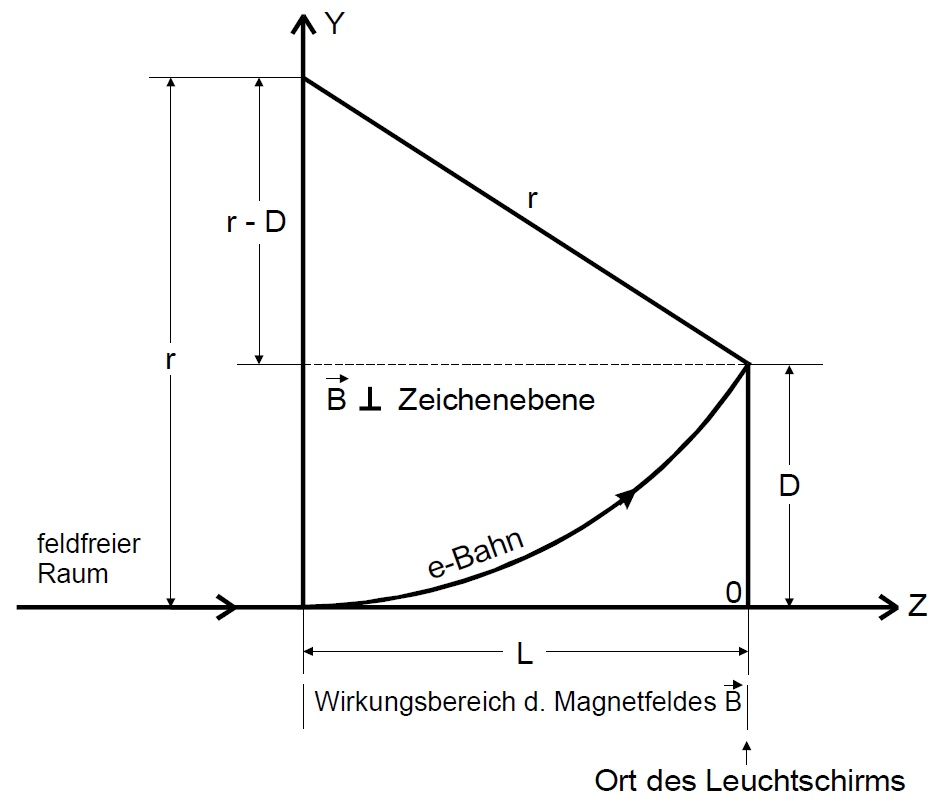
\includegraphics[width=0.7\textwidth]{Grafiken/V501(2)_Abb2.jpg}
  \caption{Skizze zur Ableitung einer Beziehung zwischen L, D und r \cite{V502}}
\end{figure}
Befindet sich ein Elektron nun in einem magnetischen Feld, wirkt auf das Elektron die Lorentz-Kraft $\vec{F}_L$:

\begin{equation}
  \vec{F} = e_0 (\vec{v} \times \vec{B})
\end{equation}

Für die Betrachtung entlang der Z-Achse gilt:

\begin{equation}
  F_L = e_0 v_0 B
\end{equation}

Wegen 

\begin{equation}
  \vec{F_L}\cdot d\vec{s} = 0
\end{equation}

gilt nun für $E_{pot} = const.$ daher gilt auch $E_{kin} = const.$
und somit:

\begin{equation}
  E_{kin} = \frac{1}{2} m_0 v^2
\end{equation}

Wenn man nun die Lorentz- und Zentripetal-Kraft gleichsetzt, gilt für den Radius $r$:

\begin{equation}
  r = \frac{m_0v_0}{e_0B}
\end{equation}

Die Verschiebung des Leuchtflecks lässt sich auch Darstellen als:

\begin{equation}
  r = \frac{L^2 + D^2}{2D}
\end{equation}

Damit gilt:

\begin{equation}
  \label{eq:Theorie_Qspez}
  \frac{L^2 + D^2}{2D} = \frac{m_0v_0}{e_0B}
\end{equation}

Hiermit lässt sich nun die spezifische Ladung $\frac{m_0}{e_0}$ bestimmen.
